\chapter{Numerical Continuation}

As stated in the previous section, we will be interested in following the solution
branches as it experiences several bifurcations. Since an analytical treatment is not
usually available for the problems studied in this work, we must resort to numerical methods.
Namely, we will implement and develop a numerical continuation algorithm. These type of methods
aim to solve a nonlinear equation or, more generally, a system of nonlinear equations in order to find the desired steady states of a dynamical system 
as parameters are changed. This task corresponds to finding the roots (zeros) of a vector function $\bm{F}$, as in Eq.~(\ref{eq:pre_nc_zeros}). 
We will assume we previously know a solution $\bm{u}_0$ for a certain parameter $\eta_0$, obtained
for example through numerical simulation.

\begin{equation}
    0 = \bm{F}(\bm{u}, \eta)
    \label{eq:pre_nc_zeros}
\end{equation}

Although there are several methods for finding the roots of a vector function,
in this thesis we will only use Newton's method because of its fast (quadratic) convergence
and simplicity. Recall that Newton's method is an iterative method that given an initial
guess $\bm{u_0}$ will perform successive iterations until a certain accuracy or tolerance
is reached. Each iteration is computed using Eqs~(\ref{eq:pre_nc_newt1}-\ref{eq:pre_nc_newt2}),
where $\matr{J}(\bm{u}_i, \eta)$ is the Jacobian of $\bm{F}$. Moreover, since we have access
to the Jacobian in Newton's method, we can track the stability of the solution and detect bifurcation
points by tracking changes in the sign of the determinant of the Jacobian.

\begin{align}
    \matr{J}(\bm{u}_i, \eta) \Delta \bm{u}_{i+1} &= - \bm{F}(\bm{u}_i, \eta) 
    \label{eq:pre_nc_newt1}
    \\
    \bm{u}_{i+1} &= \bm{u}_i + \Delta \bm{u}_{i+1}
    \label{eq:pre_nc_newt2}
\end{align}

\section{Natural parameter continuation}

The simplest way to perform numerical continuation is to fix the value of the parameter, in this case $\eta$, and solve
the equation (or system of equations) by means of Newton's method. Then, one can increase the 
parameter by a small step $\eta = \eta_0 + \Delta \eta$ and find the new solution using 
the previous solution $\bm{u_0}$ as initial guess for Newton's method. Finally, we repeat the process
until the whole solution branch has been computed. This method is usually called either {\em Natural Continuation}
or {\em Parameter Continuation} \cite{doedel2007lecture}

\begin{exmp}
    In order to illustrate the method lets consider a simple
    example: finding the homogeneous solutions to the Swift-Hohenberg equation. More specifically,
    we will look for both the stable and unstable equilibria of Eq.~(\ref{eq:pre_nc_she}).    
    \begin{equation}
        \dot{u} = \eta + \varepsilon u - u^3
        \label{eq:pre_nc_she}
    \end{equation}

    This is the same
    as to find the roots of a cubic polynomial: $F(u, \eta) = \eta + \varepsilon u - u^3 = 0$. The derivative
    can be determined easily: $J(u, \eta) = \varepsilon - 3u^2$. 
    %Moreover, when $\eta=0$, $F$ admits three distinct real solutions when
    % $\varepsilon$ is positive and one real and two complex conjugate roots when $\varepsilon$ is negative. 

    We will look at the case where $\varepsilon = 0.1$, for which the system is bistable. Indeed, if we start the algorithm
    at $\eta=-0.02$ taking as initial guess $u_0 = -0.4$ and perform a forward sweep (slowly increasing $\eta$), and then
    repeat the process backwards we obtain Fig.~(\ref{fig:pre_nc_she}).

    \begin{figure}[h]
        \centering
        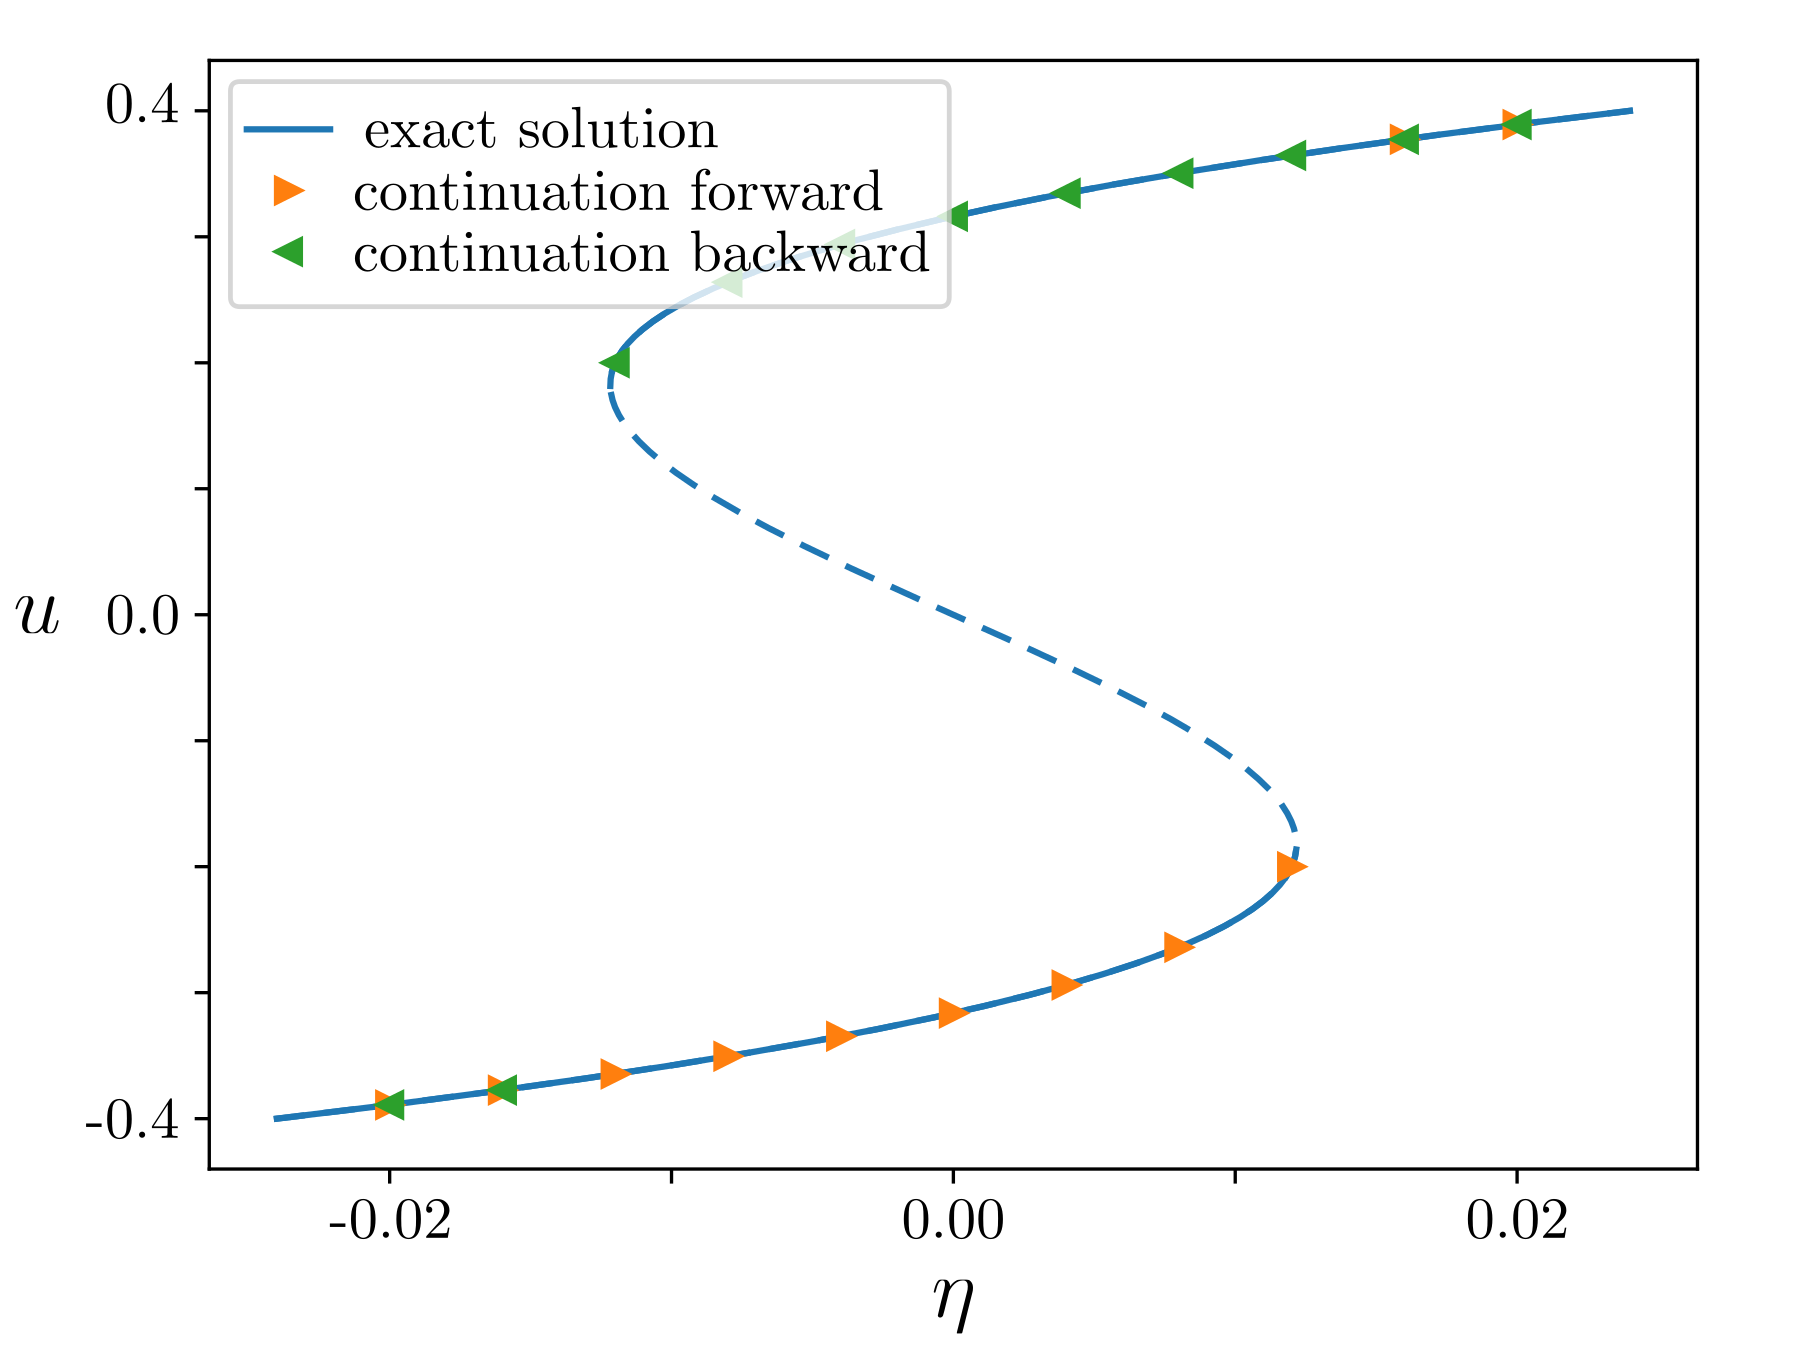
\includegraphics[width=0.7\textwidth]{scripts/figures/natural_continuation_she.png}
        \caption[short]{Solution of Eq.~(\ref{eq:pre_nc_she}) as a function of the parameter $\eta$ obtained
        through natural continuation (orange and green triangles) compared to the exact solution (blue curve).}
        \label{fig:pre_nc_she}
        %\includesvg[width=0.5\textwidth]{scripts/figures/natural_continuation_she.svg}
    \end{figure}
\end{exmp}

Note that the natural continuation succeeded at finding the lower and upper branch of the solution
in this example.
However, it could not follow the branch past the fold (or saddle-node) bifurcation. The
only way to access the middle branch using this algorithm would be to use an adequate initial guess close
to the middle branch. 
Although in this case, it is not difficult to find one, for a higher-dimensional system where the
bifurcation scenario is more complicated, this quickly becomes impractical. To overcome this limitation,
one can implement a more robust continuation scheme: the {\em pseudo-arclength continuation}.

\section{Pseudo-arclength continuation}


As shown in the previous example, $\eta$ is not necessarily the good parameter to describe the curve, as it
does not allow us to follow the branch through a fold point. A different approach can be taken where we
parametrize the solution branch by a different parameter: $s$, which is somewhat similar
to the arc-length. Therefore, our goal is to obtain a set of points 
$\bm{y}(s) = (\bm{u}(s), \eta(s))$.
Then the {\em pseudo-arclength} algorithm \cite{keller1977numerical} consists essentially of two steps that ensure that the branch is followed through folds.
\begin{enumerate}
    \item {\em Predictor step.} Extrapolate a distance $\Delta s$ along the tangent $\bm{\tau}_0$ from a previously known point $(\bm{u}_0, \eta_0)$ in the $(\bm{u},\eta)$ space, to
    obtain the predicted point (the point used as initial guess). 
    $$\bm{y} = \bm{y}_0 + \bm{\tau}_0 \Delta s$$
    \item {\em Corrector step.} Force the solution to stay in the plane perpendicular to the tangent. 
    Or, equivalently, that the solution projected onto the tangent has length $\Delta s$. 
    $$(\bm{y} - \bm{y_0}) \cdot \bm{\tau}_0 = \Delta s$$
\end{enumerate}

We have introduced in these steps a new object: the tangent $\bm{\tau}$ of the solution curve $\bm{y}(s)$,
which is defined as,
\begin{equation}
    \bm{\tau} = \frac{d}{ds}\bm{y} = \left(\frac{d\bm{u}}{ds}, \frac{d\eta}{ds}\right)
\end{equation}

An additional step must therefore be carried out in order to implement this method: computing 
the tangent vector. To do this, it is convenient to revisit Eq.~(\ref{eq:pre_nc_zeros}) and write out
the dependence on the new parameter $s$ explicitly.
\begin{equation}
    0 = \bm{F}(\bm{u}(s), \eta (s))
\end{equation}

We can take the derivative with respect to $s$ on both sides of the
above equation, and obtain the following,
\begin{equation}
    0 = \matr{J}(\bm{u}(s), \eta (s)) \frac{d \bm{u}}{ds} 
            + \bm{F_\eta}(\bm{u}(s), \eta (s)) \frac{d\eta}{ds}
   %  \matr{J}(\bm{x}(s), \eta (s))  \frac{d \bm{x}}{ds} &= -  \bm{F_\eta}(\bm{x}(s), \eta (s)) \frac{d\eta}{ds}
    \label{eq:pre_nc_tangent}
\end{equation}

Additionally, in order to uniquely define the tangent vector, we must
impose a restriction on its length, the most reasonable choice being
to normalize it. Therefore, another equation must be added,

\begin{equation}
    \left|\left|\dfrac{d\bm{u}}{ds}\right|\right|^2 + \left(\dfrac{d\eta}{ds}\right)^2 = 1
    \label{eq:pre_nc_tangent_normalization}
\end{equation}

Then, we can fix $\frac{d \eta}{ds} = 1$ and solve Eq.~(\ref{eq:pre_nc_tangent}) for $\frac{d}{ds}\bm{x}$. Since
it constitutes a system of linear equations, it can be solved using a standard linear solver. Finally, 
the tangent vector must be normalized in order to satisfy Eq.~(\ref{eq:pre_nc_tangent_normalization})
and its sign chosen such that it has the same orientation as the previously
known tangent $\bm{\tau}_0$ i.e. such that $\bm{\tau} \cdot \bm{\tau}_0 > 0$. In the very first step
of the continuation method we do not know a previous tangent, in that case we can choose the
orientation of $\bm{\tau}$ such that its last element (corresponding to  $\frac{d \eta}{ds}$) is
positive if we want to compute the solution branch for increasing values of the parameter $\eta$ or negative
for decreasing values of the parameter.

It is convenient to define an extended vector function $\tilde{ \bm{F} }$ that incorporates $\bm{F}$
and the corrector step in the following manner,
\begin{equation}
    \tilde{\bm{F}}(\bm{y}) = 
    \begin{pmatrix}
        \bm{F}(\bm{y}) \\ 
        (\bm{y} - \bm{y}_0) \cdot \bm{\tau}_0 - \Delta s
    \end{pmatrix}.
    \label{eq:pre_nc_palc_system}
\end{equation} 

And its corresponding Jacobian $\tilde{\matr{J}}$ reads
\begin{equation}
    \tilde{\matr{J}} = 
    \begin{pmatrix}
        \matr{J} & \bm{F}_\eta \\
        \dfrac{d\bm{u}}{ds} & \dfrac{d\eta}{ds} \\
    \end{pmatrix}.
\end{equation}

Notice that the last row of the extended Jacobian $\tilde{\matr{J}}$ corresponds
exactly to the tangent $\bm{\tau}$. 

We can summarize the pseudo-arclength continuation algorithm in the following steps.

\begin{enumerate}
    \item Compute a first point in the solution branch $\bm{y}_0 = (\bm{u}_0, \eta_0)$,
    typically through direct numerical simulations. Additionally, one could run
    Newton's method once while keeping the parameter fixed at $\eta = \eta_0$ to obtain
    a more accurate approximation for $\bm{u}_0$.

    \item Solve Eq.~(\ref{eq:pre_nc_tangent}) and find the tangent at that point $\bm{\tau}_0$.
    Choose the orientation of $\bm{\tau}_0$ such that it points in the desired direction on the
    $\eta$-axis.

    \item Using $\bm{y}_0 + \bm{\tau}_0 \Delta s$ as initial guess in Newton's method, solve
    Eq.~(\ref{eq:pre_nc_palc_system}) to find the next point in the solution branch $\bm{y}_{i+1}$.

    \item Again, solve Eq.~(\ref{eq:pre_nc_tangent}) and find the tangent at that point $\bm{\tau}_{i+1}$.
    Choose the orientation such that it matches the previous tangent, $\bm{\tau}_{i+1} \cdot \bm{\tau}_i > 0$.

    \item Repeat steps 3-4 until the whole solution branch has been computed. One could also
    track changes in the sign of the determinant of $\matr{J}$ in order to estimate the location
    of bifurcation points.
\end{enumerate}

% \begin{defn}[ver \cite{KAR00}] Definición definitiva $$\frac{d}{dx}\int_a^xf(y)dy=f(x).$$\end{defn}

\begin{exmp}
    Let's revisit the previous example and implement the pseudo-arclength continuation
    to the same problem. The extended function $\tilde{\bm{F}}(u, {\eta})$ can be written
    in the following form,
    \begin{equation}
        \tilde{\bm{F}}(u, \eta) = 
            \begin{pmatrix}
                \eta + \varepsilon u - u^3 \\
                \left(u - u_0\right) \dfrac{du}{ds} + (\eta - \eta_0) \dfrac{d\eta}{ds} - \Delta s
            \end{pmatrix}.
            \label{eq:pre_nc_palc_she}
    \end{equation}
    Therefore, the extended Jacobian $\tilde{\matr{J}}$ reads,
    \begin{equation*}
        \tilde{\matr{J}} = \begin{pmatrix}
                \varepsilon - 3u^2 & 1 \\
                \dfrac{du}{ds} & \dfrac{d\eta}{ds}
            \end{pmatrix}.
    \end{equation*}

    The tangent vector $\bm{\tau} = (\tau_u, \tau_{\eta})$ can be computed by solving Eq.~(\ref{eq:pre_nc_tangent}).
    We start by fixing $\frac{d}{ds}\eta = 1$, then $\frac{d}{ds}x$ can be obtained directly,
    \begin{equation*}
        \dfrac{du}{ds} = -\dfrac{F_{\eta}}{J} = -\dfrac{1}{\varepsilon - 3u^2}.
    \end{equation*}
    Finally, we normalize $\tau$ to obtain the tangent vector.

    \begin{figure}[h]
        \centering
        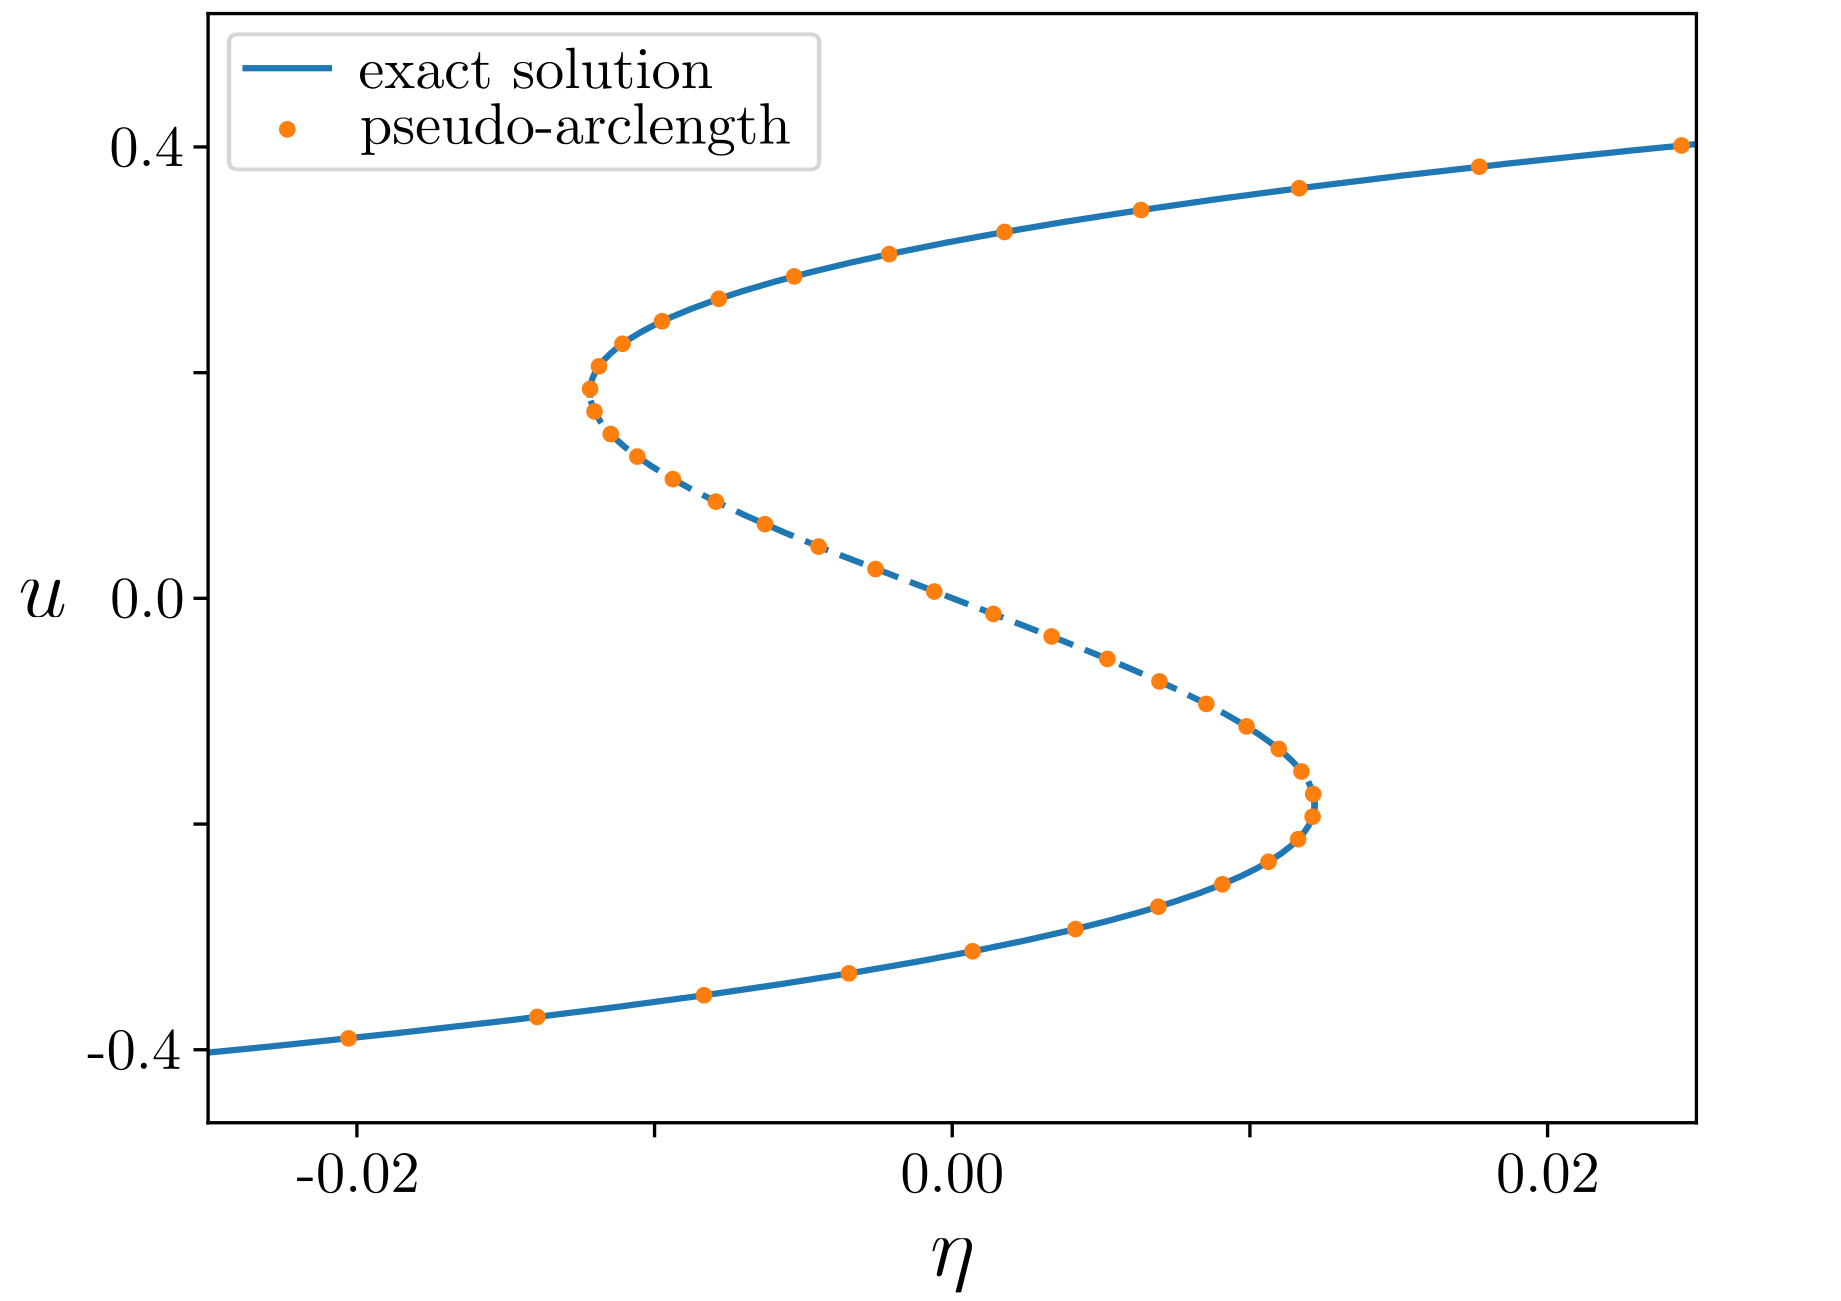
\includegraphics[width=0.7\textwidth]{scripts/figures/palc_she.png}
        \caption[short]{Solution of Eq.~(\ref{eq:pre_nc_palc_she}) as a function of the parameter $\eta$ obtained
        through the pseudo-arclength continuation (orange dots) compared to the exact solution (blue curve).}
        \label{fig:pre_nc_she}
        %\includesvg[width=0.5\textwidth]{scripts/figures/natural_continuation_she.svg}
    \end{figure}

\end{exmp}

\section{Continuation of traveling states}

In the particular case of following moving solutions with constant speed $c$, which is
the core of this work, some difficulties arise. The first and most evident one, is that
the desired solution is not steady anymore. This can be solved rather easily by
changing to the co-moving frame of reference, i.e. by inserting the traveling wave
ansatz $\bm{u}(x, t) = \bm{a}(x - ct)$, where $a$ is the solution profile in the co-moving frame,
 into Eq.~(\ref{eq:pre_nc_zeros}). Due to the chain rule,
an additional term in the form of a spatial derivative appears in the equation,

\begin{equation}
    0 = \bm{F}(\bm{a}, \eta) + c\partial_x\bm{a}
\end{equation}

The second problem is that usually the speed $c$ will change as parameters
are varied along the solution branch. Therefore, at
each step, the speed will have to be determined by the 
algorithm. The solution to this problem is to add the speed
as another unknown, that is to say, we will now be interested in solving for 
$\bm{y} = (\bm{a}, c, \eta)$. This leads to the third and final problem, which is that due
to the additional unknown, we are a missing an additional equation that will guarantee
a unique solution to the linearized system. Moreover, we will be solving these systems considering periodic
boundary conditions meaning that a translational invariance will appear. In order to
deal with the translational symmetry and guarantee a unique solution, a {\em phase condition}
or {\em pinning condition} must be established. Indeed, if we find a solution
$\bm{a}(x)$, then $\tilde{\bm{a}}_{\theta}(x) = \bm{a}(x  + \theta)$ is also
a solution for every $\theta$. 

The most widely used condition is the
{\em integral phase condition} \cite{doedel1981auto} which takes a reference solution $\bm{a}_0$ for a certain
parameter value $\eta_0$ close to the desired solution. The idea is to find the phase
that minimizes the difference $D$ between the desired solution $\bm{a}$ and the reference solution
$\bm{a}_0$. We can define the difference as follows,
\begin{equation}
    D(\theta) = \int_0^1 dx' 
        \left|\left| \bm{a}(x' + \theta) - \bm{a}_0(x') \right|\right|^2    
\end{equation}

In order to minimize the difference, we differentiate the above equation, set it equal to zero and 
then integrate by parts. Thus, we arrive at the following condition which is simpler to
implement.

\begin{equation}
    p(\bm{a}, \bm{a}_0) = \int_0^1 dx' \bm{a}(x') \cdot \left. \frac{d\bm{a}_0}{dx}\right\vert_{x'} = 0.
\end{equation}

We can re-define the extended vector function for which we want to find 
the root of in the following manner,

\begin{equation}
    \bm{H(\bm{y})} = \begin{pmatrix}
      \bm{F}(\bm{a}, \eta) + c\partial_x\bm{a} \\
    p(\bm{a}, \bm{a}_0) \\
    q(\bm{y}, \bm{y}_0)
    \end{pmatrix}
\end{equation}


The derivative of the integral phase condition with respect to the state vector $p_{\bm{a}}$ may differ depending on the chosen 
phase condition and implementation of the phase condition. In the simplest case, 
replacing the integral as a Riemann sum (which is the same as the trapezoidal rule in the case of periodic boundary conditions), the derivative reads

\begin{equation}
    p_{\bm{a}} = \Delta x \dfrac{d\bm{a}_0}{dx}.
\end{equation}

Therefore, the corresponding Jacobian of the extended function reads

\begin{equation}
    \matr{J_H}(\bm{y}) = \begin{pmatrix}
        \matr{J}(\bm{a}, \eta) + c\partial_x & \partial_x\bm{a} &  \bm{F}_\eta(\bm{a}, \eta)\\
        p_{\bm{a}}(\bm{a}_0) & 0 & 0 \\
        \dot{\bm{a}} & \dot{T} & \dot{\eta} \\
    \end{pmatrix}.
\end{equation}


\section{Continuation for periodic orbits}

If we know wish to follow periodic solutions with the continuation method we
must first derive a new set of equations to be solved. Mainly, periodic solutions
are not steady solutions of the differential equation, however they satisfy
the following boundary-value problem.

\begin{align}
    \dfrac{d\bm{u}}{dt} &= \bm{F}(\bm{u}, \eta) \\
    \bm{u}(t=0) &= \bm{u}(t=T)
\end{align}

It is convenient to rescale the time $t\to tT$, therefore the condition for
periodicity of the solution becomes $\bm{u}(t=0) = \bm{u}(t=1)$. Moreover,
due to the rescaling in time, a factor $T$ appears on the right-hand side of 
the dynamical equation. Therefore, the rescaled system becomes,

\begin{align}
    \dfrac{d\bm{u}}{dt} &= T\bm{F}(\bm{u}, \eta) \\
    \bm{u}(t=0) &= \bm{u}(t=1)
\end{align}

Moreover, due to the additional time-dependence of $\bm{u}$, the parametrizing equation for the pseudo-arclength
method needs to be modified accordingly. It now reads,

\begin{equation}
    q(\bm{y}, \bm{y}_0) = \int_0^1  (\bm{u}(t) -  \bm{u}_0(t)) \cdot \dfrac{d\bm{u}}{ds} dt 
        + (T - T_0) \dfrac{dT}{ds} + (\eta - \eta_0) \dfrac{d\eta}{ds} - \Delta s = 0 
\end{equation}

Note that we have introduced the period $T$ as another unknown which will be solved
through Newton's method along with $\bm{u}$ and $\eta$, i.e. we want to solve
for $\bm{y}(t) \equiv (\bm{u}(t), T, \eta)$. Additionally, one can add weights to the
previous equation in order to tune the search direction in Newton's method "horizontally"
(taking larger steps in the parameter $\eta$) or "vertically" (smaller steps in $\eta$),
see \cite{Uecker2017pde2path} for a more detailed discussion. Finally, we can re-define the
extended vector function for which we want to find the root of in the following manner,

\begin{equation}
    \bm{H(\bm{y})} = \begin{pmatrix}
       T \bm{F}(\bm{u}, \eta) - \frac{d\bm{u}}{dt} \\
    p(\bm{u}, \bm{u}_0) \\
    q(\bm{y}, \bm{y}_0)
    \end{pmatrix}
\end{equation}

Note that we have introduced the phase condition $p(\bm{u}, \bm{u}_0) = 0$. As stated in the previous
section, this additional equation will deal with the translational (in time) symmetry and ensure the uniqueness
of the solution.

In order to solve this system of equations subject to periodic boundary conditions, many strategies can be followed. Namely, orthogonal collocation methods
(implemented in AUTO \cite{doedel1981auto}), multiple shooting methods \cite{keller1968numerical}, and last but not least, finite difference methods
(implemented in pde2path \cite{Uecker2017pde2path}). Although the latter has the least accuracy it is by far the 
simplest to implement. In the finite difference method, a possible approximation to the
first equation in the above system is the trapezoidal rule (used for instance in the Crank-Nicolson
scheme for simulating PDEs),

\begin{equation}
    \left( \dfrac{F(\bm{u}_i) + F(\bm{u}_{i+1})}{2} \right) T 
        - \dfrac{\bm{u}_{i+1} - \bm{u}_{i}}{t_{i+1} - t_i} = 0
\end{equation}

Note that the derivative of $\bm{u}$ with respect to $t$ can be written as a product
of a matrix $\matr{\nabla}_t$ and the time-discretized vector $\bm{u}_i$ $(1 \leq i \leq n_t)$, i.e.
it can be written as $\matr{\nabla}_t\bm{u}$, in which case the Jacobian $\matr{J_H}$ of $\bm{H}$
reads

\begin{equation}
    \matr{J_H}(\bm{y}) = \begin{pmatrix}
        T \matr{J}(\bm{u}, \eta) - \matr{\nabla}_t & \bm{F}(\bm{u}, \eta) &  T\bm{F}_\eta(\bm{u}, \eta)\\
        p_{\bm{u}}(\bm{u}_0) & 0 & 0 \\
        \dot{\bm{u}} & \dot{T} & \dot{\eta} \\
    \end{pmatrix}
\end{equation}

Note that the last row corresponds, once again, exactly to the tangent vector
$\tau = (d\bm{u}/ds, dT/ds, d\eta/ds) = (\dot{\bm{u}}, \dot{T}, \dot{\eta})$.